\documentclass[1p]{elsarticle_modified}
%\bibliographystyle{elsarticle-num}

%\usepackage[colorlinks]{hyperref}
%\usepackage{abbrmath_seonhwa} %\Abb, \Ascr, \Acal ,\Abf, \Afrak
\usepackage{amsfonts}
\usepackage{amssymb}
\usepackage{amsmath}
\usepackage{amsthm}
\usepackage{scalefnt}
\usepackage{amsbsy}
\usepackage{kotex}
\usepackage{caption}
\usepackage{subfig}
\usepackage{color}
\usepackage{graphicx}
\usepackage{xcolor} %% white, black, red, green, blue, cyan, magenta, yellow
\usepackage{float}
\usepackage{setspace}
\usepackage{hyperref}

\usepackage{tikz}
\usetikzlibrary{arrows}

\usepackage{multirow}
\usepackage{array} % fixed length table
\usepackage{hhline}

%%%%%%%%%%%%%%%%%%%%%
\makeatletter
\renewcommand*\env@matrix[1][\arraystretch]{%
	\edef\arraystretch{#1}%
	\hskip -\arraycolsep
	\let\@ifnextchar\new@ifnextchar
	\array{*\c@MaxMatrixCols c}}
\makeatother %https://tex.stackexchange.com/questions/14071/how-can-i-increase-the-line-spacing-in-a-matrix
%%%%%%%%%%%%%%%

\usepackage[normalem]{ulem}

\newcommand{\msout}[1]{\ifmmode\text{\sout{\ensuremath{#1}}}\else\sout{#1}\fi}
%SOURCE: \msout is \stkout macro in https://tex.stackexchange.com/questions/20609/strikeout-in-math-mode

\newcommand{\cancel}[1]{
	\ifmmode
	{\color{red}\msout{#1}}
	\else
	{\color{red}\sout{#1}}
	\fi
}

\newcommand{\add}[1]{
	{\color{blue}\uwave{#1}}
}

\newcommand{\replace}[2]{
	\ifmmode
	{\color{red}\msout{#1}}{\color{blue}\uwave{#2}}
	\else
	{\color{red}\sout{#1}}{\color{blue}\uwave{#2}}
	\fi
}

\newcommand{\Sol}{\mathcal{S}} %segment
\newcommand{\D}{D} %diagram
\newcommand{\A}{\mathcal{A}} %arc


%%%%%%%%%%%%%%%%%%%%%%%%%%%%%5 test

\def\sl{\operatorname{\textup{SL}}(2,\Cbb)}
\def\psl{\operatorname{\textup{PSL}}(2,\Cbb)}
\def\quan{\mkern 1mu \triangleright \mkern 1mu}

\theoremstyle{definition}
\newtheorem{thm}{Theorem}[section]
\newtheorem{prop}[thm]{Proposition}
\newtheorem{lem}[thm]{Lemma}
\newtheorem{ques}[thm]{Question}
\newtheorem{cor}[thm]{Corollary}
\newtheorem{defn}[thm]{Definition}
\newtheorem{exam}[thm]{Example}
\newtheorem{rmk}[thm]{Remark}
\newtheorem{alg}[thm]{Algorithm}

\newcommand{\I}{\sqrt{-1}}
\begin{document}

%\begin{frontmatter}
%
%\title{Boundary parabolic representations of knots up to 8 crossings}
%
%%% Group authors per affiliation:
%\author{Yunhi Cho} 
%\address{Department of Mathematics, University of Seoul, Seoul, Korea}
%\ead{yhcho@uos.ac.kr}
%
%
%\author{Seonhwa Kim} %\fnref{s_kim}}
%\address{Center for Geometry and Physics, Institute for Basic Science, Pohang, 37673, Korea}
%\ead{ryeona17@ibs.re.kr}
%
%\author{Hyuk Kim}
%\address{Department of Mathematical Sciences, Seoul National University, Seoul 08826, Korea}
%\ead{hyukkim@snu.ac.kr}
%
%\author{Seokbeom Yoon}
%\address{Department of Mathematical Sciences, Seoul National University, Seoul, 08826,  Korea}
%\ead{sbyoon15@snu.ac.kr}
%
%\begin{abstract}
%We find all boundary parabolic representation of knots up to 8 crossings.
%
%\end{abstract}
%\begin{keyword}
%    \MSC[2010] 57M25 
%\end{keyword}
%
%\end{frontmatter}

%\linenumbers
%\tableofcontents
%
\newcommand\colored[1]{\textcolor{white}{\rule[-0.35ex]{0.8em}{1.4ex}}\kern-0.8em\color{red} #1}%
%\newcommand\colored[1]{\textcolor{white}{ #1}\kern-2.17ex	\textcolor{white}{ #1}\kern-1.81ex	\textcolor{white}{ #1}\kern-2.15ex\color{red}#1	}

{\Large $\underline{11a_{23}~(K11a_{23})}$}

\setlength{\tabcolsep}{10pt}
\renewcommand{\arraystretch}{1.6}
\vspace{1cm}\begin{tabular}{m{100pt}>{\centering\arraybackslash}m{274pt}}
\multirow{5}{120pt}{
	\centering
	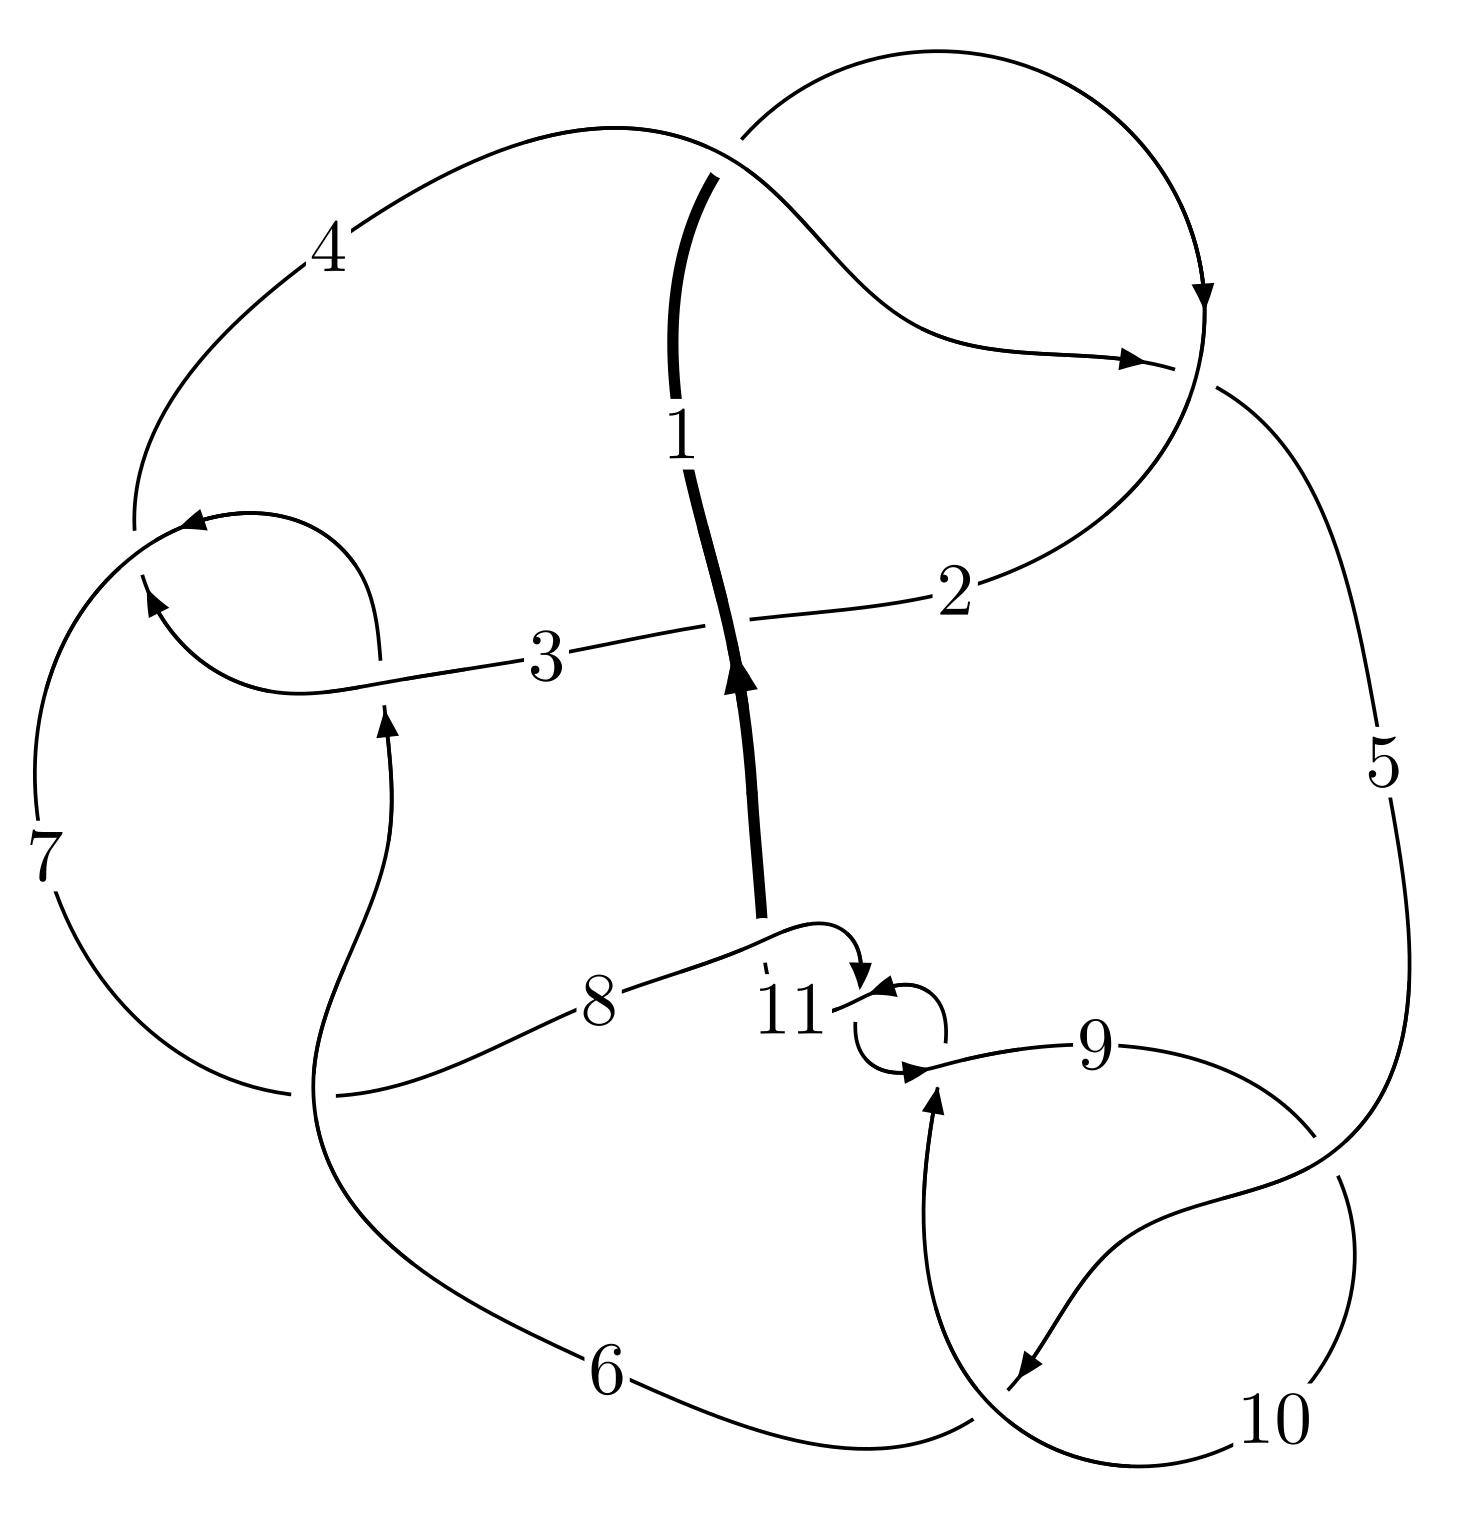
\includegraphics[width=112pt]{../../../GIT/diagram.site/Diagrams/png/272_11a_23.png}\\
\ \ \ A knot diagram\footnotemark}&
\allowdisplaybreaks
\textbf{Linearized knot diagam} \\
\cline{2-2}
 &
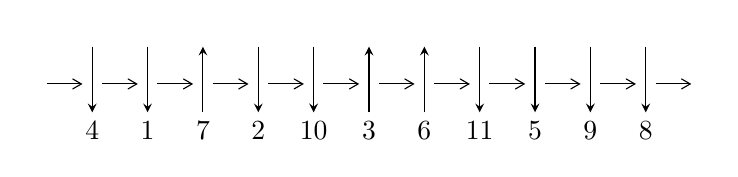
\begin{tikzpicture}[x=20pt, y=17pt]
	% nodes
	\node (C0) at (0, 0) {};
	\node (C1) at (1, 0) {};
	\node (C1U) at (1, +1) {};
	\node (C1D) at (1, -1) {4};

	\node (C2) at (2, 0) {};
	\node (C2U) at (2, +1) {};
	\node (C2D) at (2, -1) {1};

	\node (C3) at (3, 0) {};
	\node (C3U) at (3, +1) {};
	\node (C3D) at (3, -1) {7};

	\node (C4) at (4, 0) {};
	\node (C4U) at (4, +1) {};
	\node (C4D) at (4, -1) {2};

	\node (C5) at (5, 0) {};
	\node (C5U) at (5, +1) {};
	\node (C5D) at (5, -1) {10};

	\node (C6) at (6, 0) {};
	\node (C6U) at (6, +1) {};
	\node (C6D) at (6, -1) {3};

	\node (C7) at (7, 0) {};
	\node (C7U) at (7, +1) {};
	\node (C7D) at (7, -1) {6};

	\node (C8) at (8, 0) {};
	\node (C8U) at (8, +1) {};
	\node (C8D) at (8, -1) {11};

	\node (C9) at (9, 0) {};
	\node (C9U) at (9, +1) {};
	\node (C9D) at (9, -1) {5};

	\node (C10) at (10, 0) {};
	\node (C10U) at (10, +1) {};
	\node (C10D) at (10, -1) {9};

	\node (C11) at (11, 0) {};
	\node (C11U) at (11, +1) {};
	\node (C11D) at (11, -1) {8};
	\node (C12) at (12, 0) {};

	% arrows
	\draw[->,>={angle 60}]
	(C0) edge (C1) (C1) edge (C2) (C2) edge (C3) (C3) edge (C4) (C4) edge (C5) (C5) edge (C6) (C6) edge (C7) (C7) edge (C8) (C8) edge (C9) (C9) edge (C10) (C10) edge (C11) (C11) edge (C12) ;	\draw[->,>=stealth]
	(C1U) edge (C1D) (C2U) edge (C2D) (C3D) edge (C3U) (C4U) edge (C4D) (C5U) edge (C5D) (C6D) edge (C6U) (C7D) edge (C7U) (C8U) edge (C8D) (C9U) edge (C9D) (C10U) edge (C10D) (C11U) edge (C11D) ;
	\end{tikzpicture} \\
\hhline{~~} \\& 
\textbf{Solving Sequence} \\ \cline{2-2} 
 &
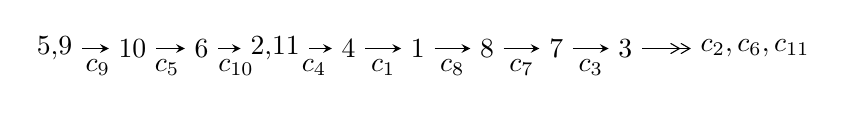
\begin{tikzpicture}[x=25pt, y=7pt]
	% node
	\node (A0) at (-1/8, 0) {5,9};
	\node (A1) at (1, 0) {10};
	\node (A2) at (2, 0) {6};
	\node (A3) at (49/16, 0) {2,11};
	\node (A4) at (33/8, 0) {4};
	\node (A5) at (41/8, 0) {1};
	\node (A6) at (49/8, 0) {8};
	\node (A7) at (57/8, 0) {7};
	\node (A8) at (65/8, 0) {3};
	\node (C1) at (1/2, -1) {$c_{9}$};
	\node (C2) at (3/2, -1) {$c_{5}$};
	\node (C3) at (5/2, -1) {$c_{10}$};
	\node (C4) at (29/8, -1) {$c_{4}$};
	\node (C5) at (37/8, -1) {$c_{1}$};
	\node (C6) at (45/8, -1) {$c_{8}$};
	\node (C7) at (53/8, -1) {$c_{7}$};
	\node (C8) at (61/8, -1) {$c_{3}$};
	\node (A9) at (10, 0) {$c_{2},c_{6},c_{11}$};

	% edge
	\draw[->,>=stealth]	
	(A0) edge (A1) (A1) edge (A2) (A2) edge (A3) (A3) edge (A4) (A4) edge (A5) (A5) edge (A6) (A6) edge (A7) (A7) edge (A8) ;
	\draw[->>,>={angle 60}]	
	(A8) edge (A9);
\end{tikzpicture} \\ 

\end{tabular} \\

\footnotetext{
The image of knot diagram is generated by the software ``\textbf{Draw programme}" developed by Andrew Bartholomew(\url{http://www.layer8.co.uk/maths/draw/index.htm\#Running-draw}), where we modified some parts for our purpose(\url{https://github.com/CATsTAILs/LinksPainter}).
}\phantom \\ \newline 
\centering \textbf{Ideals for irreducible components\footnotemark of $X_{\text{par}}$} 
 
\begin{align*}
I^u_{1}&=\langle 
u^{53}-2 u^{52}+\cdots+b+1,\;u^{52}- u^{51}+\cdots+a- u,\;u^{54}-2 u^{53}+\cdots+2 u^2-1\rangle \\
I^u_{2}&=\langle 
- u^2+b+u,\;u^2+a- u,\;u^3- u^2+1\rangle \\
\\
\end{align*}
\raggedright * 2 irreducible components of $\dim_{\mathbb{C}}=0$, with total 57 representations.\\
\footnotetext{All coefficients of polynomials are rational numbers. But the coefficients are sometimes approximated in decimal forms when there is not enough margin.}
\newpage
\renewcommand{\arraystretch}{1}
\centering \section*{I. $I^u_{1}= \langle u^{53}-2 u^{52}+\cdots+b+1,\;u^{52}- u^{51}+\cdots+a- u,\;u^{54}-2 u^{53}+\cdots+2 u^2-1 \rangle$}
\flushleft \textbf{(i) Arc colorings}\\
\begin{tabular}{m{7pt} m{180pt} m{7pt} m{180pt} }
\flushright $a_{5}=$&$\begin{pmatrix}0\\u\end{pmatrix}$ \\
\flushright $a_{9}=$&$\begin{pmatrix}1\\0\end{pmatrix}$ \\
\flushright $a_{10}=$&$\begin{pmatrix}1\\u^2\end{pmatrix}$ \\
\flushright $a_{6}=$&$\begin{pmatrix}- u\\- u^3+u\end{pmatrix}$ \\
\flushright $a_{2}=$&$\begin{pmatrix}- u^{52}+u^{51}+\cdots+7 u^3+u\\- u^{53}+2 u^{52}+\cdots-2 u-1\end{pmatrix}$ \\
\flushright $a_{11}=$&$\begin{pmatrix}- u^2+1\\u^2\end{pmatrix}$ \\
\flushright $a_{4}=$&$\begin{pmatrix}- u^{52}+u^{51}+\cdots+u-1\\u^{52}- u^{51}+\cdots- u^2- u\end{pmatrix}$ \\
\flushright $a_{1}=$&$\begin{pmatrix}- u^6+u^4-2 u^2+1\\u^6+u^2\end{pmatrix}$ \\
\flushright $a_{8}=$&$\begin{pmatrix}u^4- u^2+1\\- u^4\end{pmatrix}$ \\
\flushright $a_{7}=$&$\begin{pmatrix}u^8- u^6+3 u^4-2 u^2+1\\u^{10}-2 u^8+3 u^6-4 u^4+u^2\end{pmatrix}$ \\
\flushright $a_{3}=$&$\begin{pmatrix}- u^{52}+u^{51}+\cdots+3 u^3+2 u\\-2 u^{53}+3 u^{52}+\cdots-2 u-2\end{pmatrix}$\\ \flushright $a_{3}=$&$\begin{pmatrix}- u^{52}+u^{51}+\cdots+3 u^3+2 u\\-2 u^{53}+3 u^{52}+\cdots-2 u-2\end{pmatrix}$\\&\end{tabular}
\flushleft \textbf{(ii) Obstruction class $= -1$}\\~\\
\flushleft \textbf{(iii) Cusp Shapes $= u^{53}+2 u^{52}+\cdots-13 u-5$}\\~\\
\newpage\renewcommand{\arraystretch}{1}
\flushleft \textbf{(iv) u-Polynomials at the component}\newline \\
\begin{tabular}{m{50pt}|m{274pt}}
Crossings & \hspace{64pt}u-Polynomials at each crossing \\
\hline $$\begin{aligned}c_{1},c_{4}\end{aligned}$$&$\begin{aligned}
&u^{54}-4 u^{53}+\cdots+5 u-1
\end{aligned}$\\
\hline $$\begin{aligned}c_{2}\end{aligned}$$&$\begin{aligned}
&u^{54}+28 u^{53}+\cdots+5 u+1
\end{aligned}$\\
\hline $$\begin{aligned}c_{3},c_{6}\end{aligned}$$&$\begin{aligned}
&u^{54}- u^{53}+\cdots+28 u+8
\end{aligned}$\\
\hline $$\begin{aligned}c_{5},c_{9}\end{aligned}$$&$\begin{aligned}
&u^{54}+2 u^{53}+\cdots+2 u^2-1
\end{aligned}$\\
\hline $$\begin{aligned}c_{7}\end{aligned}$$&$\begin{aligned}
&u^{54}-21 u^{53}+\cdots-912 u+64
\end{aligned}$\\
\hline $$\begin{aligned}c_{8},c_{10},c_{11}\end{aligned}$$&$\begin{aligned}
&u^{54}+14 u^{53}+\cdots+4 u+1
\end{aligned}$\\
\hline
\end{tabular}\\~\\
\newpage\renewcommand{\arraystretch}{1}
\flushleft \textbf{(v) Riley Polynomials at the component}\newline \\
\begin{tabular}{m{50pt}|m{274pt}}
Crossings & \hspace{64pt}Riley Polynomials at each crossing \\
\hline $$\begin{aligned}c_{1},c_{4}\end{aligned}$$&$\begin{aligned}
&y^{54}-28 y^{53}+\cdots-5 y+1
\end{aligned}$\\
\hline $$\begin{aligned}c_{2}\end{aligned}$$&$\begin{aligned}
&y^{54}+44 y^{52}+\cdots-29 y+1
\end{aligned}$\\
\hline $$\begin{aligned}c_{3},c_{6}\end{aligned}$$&$\begin{aligned}
&y^{54}-21 y^{53}+\cdots-912 y+64
\end{aligned}$\\
\hline $$\begin{aligned}c_{5},c_{9}\end{aligned}$$&$\begin{aligned}
&y^{54}-14 y^{53}+\cdots-4 y+1
\end{aligned}$\\
\hline $$\begin{aligned}c_{7}\end{aligned}$$&$\begin{aligned}
&y^{54}+19 y^{53}+\cdots-85248 y+4096
\end{aligned}$\\
\hline $$\begin{aligned}c_{8},c_{10},c_{11}\end{aligned}$$&$\begin{aligned}
&y^{54}+54 y^{53}+\cdots-28 y+1
\end{aligned}$\\
\hline
\end{tabular}\\~\\
\newpage\flushleft \textbf{(vi) Complex Volumes and Cusp Shapes}
$$\begin{array}{c|c|c}  
\text{Solutions to }I^u_{1}& \I (\text{vol} + \sqrt{-1}CS) & \text{Cusp shape}\\
 \hline 
\begin{aligned}
u &= \phantom{-}0.948112 + 0.298354 I \\
a &= \phantom{-}1.205050 + 0.065806 I \\
b &= -2.47632 + 1.36880 I\end{aligned}
 & -4.67558 - 3.96496 I & -10.65253 + 5.36076 I \\ \hline\begin{aligned}
u &= \phantom{-}0.948112 - 0.298354 I \\
a &= \phantom{-}1.205050 - 0.065806 I \\
b &= -2.47632 - 1.36880 I\end{aligned}
 & -4.67558 + 3.96496 I & -10.65253 - 5.36076 I \\ \hline\begin{aligned}
u &= -0.718756 + 0.708822 I \\
a &= \phantom{-}0.989080 + 0.349916 I \\
b &= -0.893237 - 0.687723 I\end{aligned}
 & \phantom{-}1.72344 + 4.24877 I & -1.89208 - 7.05777 I \\ \hline\begin{aligned}
u &= -0.718756 - 0.708822 I \\
a &= \phantom{-}0.989080 - 0.349916 I \\
b &= -0.893237 + 0.687723 I\end{aligned}
 & \phantom{-}1.72344 - 4.24877 I & -1.89208 + 7.05777 I \\ \hline\begin{aligned}
u &= -0.953732 + 0.349837 I \\
a &= -0.061370 + 0.782367 I \\
b &= \phantom{-}0.558618 - 0.498636 I\end{aligned}
 & -0.69346 + 4.89748 I & -4.90328 - 6.49260 I \\ \hline\begin{aligned}
u &= -0.953732 - 0.349837 I \\
a &= -0.061370 - 0.782367 I \\
b &= \phantom{-}0.558618 + 0.498636 I\end{aligned}
 & -0.69346 - 4.89748 I & -4.90328 + 6.49260 I \\ \hline\begin{aligned}
u &= -0.829612 + 0.586776 I \\
a &= \phantom{-}0.900184 + 0.101382 I \\
b &= -1.216120 - 0.670600 I\end{aligned}
 & \phantom{-}1.80763 + 4.19776 I & -1.27767 - 7.87465 I \\ \hline\begin{aligned}
u &= -0.829612 - 0.586776 I \\
a &= \phantom{-}0.900184 - 0.101382 I \\
b &= -1.216120 + 0.670600 I\end{aligned}
 & \phantom{-}1.80763 - 4.19776 I & -1.27767 + 7.87465 I \\ \hline\begin{aligned}
u &= \phantom{-}1.006640 + 0.186947 I \\
a &= -0.985399 + 0.649993 I \\
b &= \phantom{-}1.58875 - 0.30591 I\end{aligned}
 & -4.34560 + 3.65314 I & -10.05122 - 3.06776 I \\ \hline\begin{aligned}
u &= \phantom{-}1.006640 - 0.186947 I \\
a &= -0.985399 - 0.649993 I \\
b &= \phantom{-}1.58875 + 0.30591 I\end{aligned}
 & -4.34560 - 3.65314 I & -10.05122 + 3.06776 I\\
 \hline 
 \end{array}$$\newpage$$\begin{array}{c|c|c}  
\text{Solutions to }I^u_{1}& \I (\text{vol} + \sqrt{-1}CS) & \text{Cusp shape}\\
 \hline 
\begin{aligned}
u &= -0.936944 + 0.259765 I \\
a &= -1.088760 - 0.644557 I \\
b &= \phantom{-}1.68766 + 0.11648 I\end{aligned}
 & -4.90867 + 1.39018 I & -11.17255 - 4.35263 I \\ \hline\begin{aligned}
u &= -0.936944 - 0.259765 I \\
a &= -1.088760 + 0.644557 I \\
b &= \phantom{-}1.68766 - 0.11648 I\end{aligned}
 & -4.90867 - 1.39018 I & -11.17255 + 4.35263 I \\ \hline\begin{aligned}
u &= -1.007510 + 0.341711 I \\
a &= \phantom{-}1.191860 - 0.125655 I \\
b &= -2.43976 - 0.96569 I\end{aligned}
 & -3.43639 + 9.75051 I & -8.30305 - 9.36472 I \\ \hline\begin{aligned}
u &= -1.007510 - 0.341711 I \\
a &= \phantom{-}1.191860 + 0.125655 I \\
b &= -2.43976 + 0.96569 I\end{aligned}
 & -3.43639 - 9.75051 I & -8.30305 + 9.36472 I \\ \hline\begin{aligned}
u &= \phantom{-}0.892491 + 0.183773 I \\
a &= -0.171964 - 0.552035 I \\
b &= \phantom{-}0.779603 + 0.338273 I\end{aligned}
 & -1.67290 - 0.31402 I & -7.28536 + 0.85083 I \\ \hline\begin{aligned}
u &= \phantom{-}0.892491 - 0.183773 I \\
a &= -0.171964 + 0.552035 I \\
b &= \phantom{-}0.779603 - 0.338273 I\end{aligned}
 & -1.67290 + 0.31402 I & -7.28536 - 0.85083 I \\ \hline\begin{aligned}
u &= \phantom{-}0.880753\phantom{ +0.000000I} \\
a &= -0.535851\phantom{ +0.000000I} \\
b &= \phantom{-}1.06380\phantom{ +0.000000I}\end{aligned}
 & -1.51820\phantom{ +0.000000I} & -5.33260\phantom{ +0.000000I} \\ \hline\begin{aligned}
u &= \phantom{-}0.831263 + 0.825334 I \\
a &= \phantom{-}0.897031 - 0.632195 I \\
b &= -0.774607 + 0.728358 I\end{aligned}
 & \phantom{-}1.86207 - 0.72710 I & -3.27217 + 0. I\phantom{ +0.000000I} \\ \hline\begin{aligned}
u &= \phantom{-}0.831263 - 0.825334 I \\
a &= \phantom{-}0.897031 + 0.632195 I \\
b &= -0.774607 - 0.728358 I\end{aligned}
 & \phantom{-}1.86207 + 0.72710 I & -3.27217 + 0. I\phantom{ +0.000000I} \\ \hline\begin{aligned}
u &= -0.823137 + 0.844727 I \\
a &= -0.312862 - 0.944385 I \\
b &= -1.73844 - 0.80253 I\end{aligned}
 & \phantom{-}2.56847 - 1.88759 I & \phantom{-0.000000 } 0\\
 \hline 
 \end{array}$$\newpage$$\begin{array}{c|c|c}  
\text{Solutions to }I^u_{1}& \I (\text{vol} + \sqrt{-1}CS) & \text{Cusp shape}\\
 \hline 
\begin{aligned}
u &= -0.823137 - 0.844727 I \\
a &= -0.312862 + 0.944385 I \\
b &= -1.73844 + 0.80253 I\end{aligned}
 & \phantom{-}2.56847 + 1.88759 I & \phantom{-0.000000 } 0 \\ \hline\begin{aligned}
u &= -0.862381 + 0.818968 I \\
a &= -0.583547 + 0.090309 I \\
b &= \phantom{-}0.49799 + 1.75744 I\end{aligned}
 & \phantom{-}4.38756 + 2.45269 I & \phantom{-0.000000 } 0 \\ \hline\begin{aligned}
u &= -0.862381 - 0.818968 I \\
a &= -0.583547 - 0.090309 I \\
b &= \phantom{-}0.49799 - 1.75744 I\end{aligned}
 & \phantom{-}4.38756 - 2.45269 I & \phantom{-0.000000 } 0 \\ \hline\begin{aligned}
u &= \phantom{-}0.804605 + 0.877981 I \\
a &= -0.294081 + 1.060590 I \\
b &= -1.35489 + 0.61945 I\end{aligned}
 & \phantom{-}4.52521 + 8.09679 I & \phantom{-0.000000 } 0 \\ \hline\begin{aligned}
u &= \phantom{-}0.804605 - 0.877981 I \\
a &= -0.294081 - 1.060590 I \\
b &= -1.35489 - 0.61945 I\end{aligned}
 & \phantom{-}4.52521 - 8.09679 I & \phantom{-0.000000 } 0 \\ \hline\begin{aligned}
u &= -0.956300 + 0.721294 I \\
a &= \phantom{-}0.490288 + 0.770861 I \\
b &= -0.371501 - 0.639488 I\end{aligned}
 & \phantom{-}1.09373 + 1.25845 I & \phantom{-0.000000 } 0 \\ \hline\begin{aligned}
u &= -0.956300 - 0.721294 I \\
a &= \phantom{-}0.490288 - 0.770861 I \\
b &= -0.371501 + 0.639488 I\end{aligned}
 & \phantom{-}1.09373 - 1.25845 I & \phantom{-0.000000 } 0 \\ \hline\begin{aligned}
u &= \phantom{-}0.826228 + 0.868166 I \\
a &= -0.706693 - 0.315162 I \\
b &= \phantom{-}0.91045 - 1.19576 I\end{aligned}
 & \phantom{-}7.09944 + 2.70045 I & \phantom{-0.000000 } 0 \\ \hline\begin{aligned}
u &= \phantom{-}0.826228 - 0.868166 I \\
a &= -0.706693 + 0.315162 I \\
b &= \phantom{-}0.91045 + 1.19576 I\end{aligned}
 & \phantom{-}7.09944 - 2.70045 I & \phantom{-0.000000 } 0 \\ \hline\begin{aligned}
u &= -0.926090 + 0.797649 I \\
a &= \phantom{-}0.083529 - 0.557091 I \\
b &= -1.82650 + 0.41695 I\end{aligned}
 & \phantom{-}4.18784 + 3.59964 I & \phantom{-0.000000 } 0\\
 \hline 
 \end{array}$$\newpage$$\begin{array}{c|c|c}  
\text{Solutions to }I^u_{1}& \I (\text{vol} + \sqrt{-1}CS) & \text{Cusp shape}\\
 \hline 
\begin{aligned}
u &= -0.926090 - 0.797649 I \\
a &= \phantom{-}0.083529 + 0.557091 I \\
b &= -1.82650 - 0.41695 I\end{aligned}
 & \phantom{-}4.18784 - 3.59964 I & \phantom{-0.000000 } 0 \\ \hline\begin{aligned}
u &= -0.516406 + 0.577695 I \\
a &= -0.036990 + 1.075540 I \\
b &= \phantom{-}0.657739 + 0.015042 I\end{aligned}
 & \phantom{-}2.66225 + 0.01615 I & \phantom{-}2.03217 - 0.16196 I \\ \hline\begin{aligned}
u &= -0.516406 - 0.577695 I \\
a &= -0.036990 - 1.075540 I \\
b &= \phantom{-}0.657739 - 0.015042 I\end{aligned}
 & \phantom{-}2.66225 - 0.01615 I & \phantom{-}2.03217 + 0.16196 I \\ \hline\begin{aligned}
u &= \phantom{-}0.950127 + 0.790670 I \\
a &= \phantom{-}0.667535 - 0.810906 I \\
b &= -0.527757 + 0.770419 I\end{aligned}
 & \phantom{-}1.49449 - 5.32145 I & \phantom{-0.000000 } 0 \\ \hline\begin{aligned}
u &= \phantom{-}0.950127 - 0.790670 I \\
a &= \phantom{-}0.667535 + 0.810906 I \\
b &= -0.527757 - 0.770419 I\end{aligned}
 & \phantom{-}1.49449 + 5.32145 I & \phantom{-0.000000 } 0 \\ \hline\begin{aligned}
u &= \phantom{-}0.896659 + 0.861407 I \\
a &= -0.040376 + 0.871785 I \\
b &= -1.82541 + 0.01530 I\end{aligned}
 & \phantom{-}9.95886 - 0.40591 I & \phantom{-0.000000 } 0 \\ \hline\begin{aligned}
u &= \phantom{-}0.896659 - 0.861407 I \\
a &= -0.040376 - 0.871785 I \\
b &= -1.82541 - 0.01530 I\end{aligned}
 & \phantom{-}9.95886 + 0.40591 I & \phantom{-0.000000 } 0 \\ \hline\begin{aligned}
u &= -0.962624 + 0.798447 I \\
a &= -0.928929 - 0.233282 I \\
b &= \phantom{-}2.53779 + 2.34211 I\end{aligned}
 & \phantom{-}2.13549 + 8.01692 I & \phantom{-0.000000 } 0 \\ \hline\begin{aligned}
u &= -0.962624 - 0.798447 I \\
a &= -0.928929 + 0.233282 I \\
b &= \phantom{-}2.53779 - 2.34211 I\end{aligned}
 & \phantom{-}2.13549 - 8.01692 I & \phantom{-0.000000 } 0 \\ \hline\begin{aligned}
u &= \phantom{-}0.923219 + 0.851100 I \\
a &= -0.876432 + 0.007481 I \\
b &= \phantom{-}1.57894 - 1.93563 I\end{aligned}
 & \phantom{-}9.87556 - 5.94354 I & \phantom{-0.000000 } 0\\
 \hline 
 \end{array}$$\newpage$$\begin{array}{c|c|c}  
\text{Solutions to }I^u_{1}& \I (\text{vol} + \sqrt{-1}CS) & \text{Cusp shape}\\
 \hline 
\begin{aligned}
u &= \phantom{-}0.923219 - 0.851100 I \\
a &= -0.876432 - 0.007481 I \\
b &= \phantom{-}1.57894 + 1.93563 I\end{aligned}
 & \phantom{-}9.87556 + 5.94354 I & \phantom{-0.000000 } 0 \\ \hline\begin{aligned}
u &= \phantom{-}0.972034 + 0.812571 I \\
a &= \phantom{-}0.275106 + 0.680780 I \\
b &= -1.73893 - 0.27634 I\end{aligned}
 & \phantom{-}6.64241 - 8.94495 I & \phantom{-0.000000 } 0 \\ \hline\begin{aligned}
u &= \phantom{-}0.972034 - 0.812571 I \\
a &= \phantom{-}0.275106 - 0.680780 I \\
b &= -1.73893 + 0.27634 I\end{aligned}
 & \phantom{-}6.64241 + 8.94495 I & \phantom{-0.000000 } 0 \\ \hline\begin{aligned}
u &= \phantom{-}0.988340 + 0.806697 I \\
a &= -1.009690 + 0.227138 I \\
b &= \phantom{-}2.56726 - 1.93517 I\end{aligned}
 & \phantom{-}3.9497 - 14.3488 I & \phantom{-0.000000 } 0 \\ \hline\begin{aligned}
u &= \phantom{-}0.988340 - 0.806697 I \\
a &= -1.009690 - 0.227138 I \\
b &= \phantom{-}2.56726 + 1.93517 I\end{aligned}
 & \phantom{-}3.9497 + 14.3488 I & \phantom{-0.000000 } 0 \\ \hline\begin{aligned}
u &= -0.137568 + 0.670291 I \\
a &= -0.44103 + 1.74491 I \\
b &= \phantom{-}0.799841 - 0.000276 I\end{aligned}
 & -0.68378 - 6.18510 I & -2.38929 + 5.41509 I \\ \hline\begin{aligned}
u &= -0.137568 - 0.670291 I \\
a &= -0.44103 - 1.74491 I \\
b &= \phantom{-}0.799841 + 0.000276 I\end{aligned}
 & -0.68378 + 6.18510 I & -2.38929 - 5.41509 I \\ \hline\begin{aligned}
u &= \phantom{-}0.571380 + 0.287951 I \\
a &= \phantom{-}1.207730 - 0.200032 I \\
b &= \phantom{-}0.06093 + 1.45702 I\end{aligned}
 & -1.12376 - 1.18488 I & -5.58028 + 5.43531 I \\ \hline\begin{aligned}
u &= \phantom{-}0.571380 - 0.287951 I \\
a &= \phantom{-}1.207730 + 0.200032 I \\
b &= \phantom{-}0.06093 - 1.45702 I\end{aligned}
 & -1.12376 + 1.18488 I & -5.58028 - 5.43531 I \\ \hline\begin{aligned}
u &= -0.211819 + 0.582109 I \\
a &= \phantom{-}1.207330 + 0.116243 I \\
b &= -0.531021 - 0.291086 I\end{aligned}
 & \phantom{-}1.59069 - 1.49648 I & \phantom{-}1.55257 + 1.21320 I\\
 \hline 
 \end{array}$$\newpage$$\begin{array}{c|c|c}  
\text{Solutions to }I^u_{1}& \I (\text{vol} + \sqrt{-1}CS) & \text{Cusp shape}\\
 \hline 
\begin{aligned}
u &= -0.211819 - 0.582109 I \\
a &= \phantom{-}1.207330 - 0.116243 I \\
b &= -0.531021 + 0.291086 I\end{aligned}
 & \phantom{-}1.59069 + 1.49648 I & \phantom{-}1.55257 - 1.21320 I \\ \hline\begin{aligned}
u &= -0.567584\phantom{ +0.000000I} \\
a &= -1.94525\phantom{ +0.000000I} \\
b &= \phantom{-}1.23770\phantom{ +0.000000I}\end{aligned}
 & -2.29901\phantom{ +0.000000I} & \phantom{-}2.64120\phantom{ +0.000000I} \\ \hline\begin{aligned}
u &= \phantom{-}0.075195 + 0.497044 I \\
a &= -0.33607 - 2.18707 I \\
b &= \phantom{-}0.838168 - 0.011197 I\end{aligned}
 & -2.17031 + 1.07616 I & -4.84925 - 0.51569 I \\ \hline\begin{aligned}
u &= \phantom{-}0.075195 - 0.497044 I \\
a &= -0.33607 + 2.18707 I \\
b &= \phantom{-}0.838168 + 0.011197 I\end{aligned}
 & -2.17031 - 1.07616 I & -4.84925 + 0.51569 I\\
 \hline 
 \end{array}$$\newpage\newpage\renewcommand{\arraystretch}{1}
\centering \section*{II. $I^u_{2}= \langle - u^2+b+u,\;u^2+a- u,\;u^3- u^2+1 \rangle$}
\flushleft \textbf{(i) Arc colorings}\\
\begin{tabular}{m{7pt} m{180pt} m{7pt} m{180pt} }
\flushright $a_{5}=$&$\begin{pmatrix}0\\u\end{pmatrix}$ \\
\flushright $a_{9}=$&$\begin{pmatrix}1\\0\end{pmatrix}$ \\
\flushright $a_{10}=$&$\begin{pmatrix}1\\u^2\end{pmatrix}$ \\
\flushright $a_{6}=$&$\begin{pmatrix}- u\\- u^2+u+1\end{pmatrix}$ \\
\flushright $a_{2}=$&$\begin{pmatrix}- u^2+u\\u^2- u\end{pmatrix}$ \\
\flushright $a_{11}=$&$\begin{pmatrix}- u^2+1\\u^2\end{pmatrix}$ \\
\flushright $a_{4}=$&$\begin{pmatrix}- u^2+u\\u^2\end{pmatrix}$ \\
\flushright $a_{1}=$&$\begin{pmatrix}0\\- u\end{pmatrix}$ \\
\flushright $a_{8}=$&$\begin{pmatrix}- u\\- u^2+u+1\end{pmatrix}$ \\
\flushright $a_{7}=$&$\begin{pmatrix}- u\\- u^2+u+1\end{pmatrix}$ \\
\flushright $a_{3}=$&$\begin{pmatrix}- u^2+u\\u^2\end{pmatrix}$\\ \flushright $a_{3}=$&$\begin{pmatrix}- u^2+u\\u^2\end{pmatrix}$\\&\end{tabular}
\flushleft \textbf{(ii) Obstruction class $= 1$}\\~\\
\flushleft \textbf{(iii) Cusp Shapes $= -2 u^2+7 u-10$}\\~\\
\newpage\renewcommand{\arraystretch}{1}
\flushleft \textbf{(iv) u-Polynomials at the component}\newline \\
\begin{tabular}{m{50pt}|m{274pt}}
Crossings & \hspace{64pt}u-Polynomials at each crossing \\
\hline $$\begin{aligned}c_{1}\end{aligned}$$&$\begin{aligned}
&(u-1)^3
\end{aligned}$\\
\hline $$\begin{aligned}c_{2},c_{4}\end{aligned}$$&$\begin{aligned}
&(u+1)^3
\end{aligned}$\\
\hline $$\begin{aligned}c_{3},c_{6},c_{7}\end{aligned}$$&$\begin{aligned}
&u^3
\end{aligned}$\\
\hline $$\begin{aligned}c_{5}\end{aligned}$$&$\begin{aligned}
&u^3+u^2-1
\end{aligned}$\\
\hline $$\begin{aligned}c_{8}\end{aligned}$$&$\begin{aligned}
&u^3- u^2+2 u-1
\end{aligned}$\\
\hline $$\begin{aligned}c_{9}\end{aligned}$$&$\begin{aligned}
&u^3- u^2+1
\end{aligned}$\\
\hline $$\begin{aligned}c_{10},c_{11}\end{aligned}$$&$\begin{aligned}
&u^3+u^2+2 u+1
\end{aligned}$\\
\hline
\end{tabular}\\~\\
\newpage\renewcommand{\arraystretch}{1}
\flushleft \textbf{(v) Riley Polynomials at the component}\newline \\
\begin{tabular}{m{50pt}|m{274pt}}
Crossings & \hspace{64pt}Riley Polynomials at each crossing \\
\hline $$\begin{aligned}c_{1},c_{2},c_{4}\end{aligned}$$&$\begin{aligned}
&(y-1)^3
\end{aligned}$\\
\hline $$\begin{aligned}c_{3},c_{6},c_{7}\end{aligned}$$&$\begin{aligned}
&y^3
\end{aligned}$\\
\hline $$\begin{aligned}c_{5},c_{9}\end{aligned}$$&$\begin{aligned}
&y^3- y^2+2 y-1
\end{aligned}$\\
\hline $$\begin{aligned}c_{8},c_{10},c_{11}\end{aligned}$$&$\begin{aligned}
&y^3+3 y^2+2 y-1
\end{aligned}$\\
\hline
\end{tabular}\\~\\
\newpage\flushleft \textbf{(vi) Complex Volumes and Cusp Shapes}
$$\begin{array}{c|c|c}  
\text{Solutions to }I^u_{2}& \I (\text{vol} + \sqrt{-1}CS) & \text{Cusp shape}\\
 \hline 
\begin{aligned}
u &= \phantom{-}0.877439 + 0.744862 I \\
a &= \phantom{-}0.662359 - 0.562280 I \\
b &= -0.662359 + 0.562280 I\end{aligned}
 & \phantom{-}1.37919 - 2.82812 I & -4.28809 + 2.59975 I \\ \hline\begin{aligned}
u &= \phantom{-}0.877439 - 0.744862 I \\
a &= \phantom{-}0.662359 + 0.562280 I \\
b &= -0.662359 - 0.562280 I\end{aligned}
 & \phantom{-}1.37919 + 2.82812 I & -4.28809 - 2.59975 I \\ \hline\begin{aligned}
u &= -0.754878\phantom{ +0.000000I} \\
a &= -1.32472\phantom{ +0.000000I} \\
b &= \phantom{-}1.32472\phantom{ +0.000000I}\end{aligned}
 & -2.75839\phantom{ +0.000000I} & -16.4240\phantom{ +0.000000I}\\
 \hline 
 \end{array}$$\newpage
\newpage\renewcommand{\arraystretch}{1}
\centering \section*{ III. u-Polynomials}
\begin{tabular}{m{50pt}|m{274pt}}
Crossings & \hspace{64pt}u-Polynomials at each crossing \\
\hline $$\begin{aligned}c_{1}\end{aligned}$$&$\begin{aligned}
&((u-1)^3)(u^{54}-4 u^{53}+\cdots+5 u-1)
\end{aligned}$\\
\hline $$\begin{aligned}c_{2}\end{aligned}$$&$\begin{aligned}
&((u+1)^3)(u^{54}+28 u^{53}+\cdots+5 u+1)
\end{aligned}$\\
\hline $$\begin{aligned}c_{3},c_{6}\end{aligned}$$&$\begin{aligned}
&u^3(u^{54}- u^{53}+\cdots+28 u+8)
\end{aligned}$\\
\hline $$\begin{aligned}c_{4}\end{aligned}$$&$\begin{aligned}
&((u+1)^3)(u^{54}-4 u^{53}+\cdots+5 u-1)
\end{aligned}$\\
\hline $$\begin{aligned}c_{5}\end{aligned}$$&$\begin{aligned}
&(u^3+u^2-1)(u^{54}+2 u^{53}+\cdots+2 u^2-1)
\end{aligned}$\\
\hline $$\begin{aligned}c_{7}\end{aligned}$$&$\begin{aligned}
&u^3(u^{54}-21 u^{53}+\cdots-912 u+64)
\end{aligned}$\\
\hline $$\begin{aligned}c_{8}\end{aligned}$$&$\begin{aligned}
&(u^3- u^2+2 u-1)(u^{54}+14 u^{53}+\cdots+4 u+1)
\end{aligned}$\\
\hline $$\begin{aligned}c_{9}\end{aligned}$$&$\begin{aligned}
&(u^3- u^2+1)(u^{54}+2 u^{53}+\cdots+2 u^2-1)
\end{aligned}$\\
\hline $$\begin{aligned}c_{10},c_{11}\end{aligned}$$&$\begin{aligned}
&(u^3+u^2+2 u+1)(u^{54}+14 u^{53}+\cdots+4 u+1)
\end{aligned}$\\
\hline
\end{tabular}\newpage\renewcommand{\arraystretch}{1}
\centering \section*{ IV. Riley Polynomials}
\begin{tabular}{m{50pt}|m{274pt}}
Crossings & \hspace{64pt}Riley Polynomials at each crossing \\
\hline $$\begin{aligned}c_{1},c_{4}\end{aligned}$$&$\begin{aligned}
&((y-1)^3)(y^{54}-28 y^{53}+\cdots-5 y+1)
\end{aligned}$\\
\hline $$\begin{aligned}c_{2}\end{aligned}$$&$\begin{aligned}
&((y-1)^3)(y^{54}+44 y^{52}+\cdots-29 y+1)
\end{aligned}$\\
\hline $$\begin{aligned}c_{3},c_{6}\end{aligned}$$&$\begin{aligned}
&y^3(y^{54}-21 y^{53}+\cdots-912 y+64)
\end{aligned}$\\
\hline $$\begin{aligned}c_{5},c_{9}\end{aligned}$$&$\begin{aligned}
&(y^3- y^2+2 y-1)(y^{54}-14 y^{53}+\cdots-4 y+1)
\end{aligned}$\\
\hline $$\begin{aligned}c_{7}\end{aligned}$$&$\begin{aligned}
&y^3(y^{54}+19 y^{53}+\cdots-85248 y+4096)
\end{aligned}$\\
\hline $$\begin{aligned}c_{8},c_{10},c_{11}\end{aligned}$$&$\begin{aligned}
&(y^3+3 y^2+2 y-1)(y^{54}+54 y^{53}+\cdots-28 y+1)
\end{aligned}$\\
\hline
\end{tabular}
\vskip 2pc
\end{document}